\documentclass[11pt,a4paper]{article}
\usepackage{fontspec}
\setmainfont{AR PL UKai CN} 
\usepackage{fontspec}
\usepackage{xunicode}
\usepackage{xltxtra}
\usepackage{indentfirst}
\XeTeXlinebreaklocale “zh”
\XeTeXlinebreakskip = 0pt plus 1pt minus 0.1pt

\usepackage{ifxetex,ifluatex}
\ifxetex
  \usepackage{fontspec,xltxtra,xunicode}
  \defaultfontfeatures{Mapping=tex-text,Scale=MatchLowercase}
\else
  \ifluatex
    \usepackage{fontspec}
    \defaultfontfeatures{Mapping=tex-text,Scale=MatchLowercase}
  \else
    \usepackage[utf8]{inputenc}
  \fi
\fi
\usepackage{url}
\usepackage{graphicx}
% We will generate all images so they have a width \maxwidth. This means
% that they will get their normal width if they fit onto the page, but
% are scaled down if they would overflow the margins.
\makeatletter
\def\maxwidth{\ifdim\Gin@nat@width>\linewidth\linewidth
\else\Gin@nat@width\fi}
\makeatother
\let\Oldincludegraphics\includegraphics
\renewcommand{\includegraphics}[1]{\Oldincludegraphics[width=\maxwidth]{#1}}
\ifxetex
  \usepackage[setpagesize=false, % page size defined by xetex
              unicode=false, % unicode breaks when used with xetex
              xetex,
              colorlinks=true,
              linkcolor=blue]{hyperref}
\else
  \usepackage[unicode=true,
              colorlinks=true,
              linkcolor=blue]{hyperref}
\fi
\hypersetup{breaklinks=true, pdfborder={0 0 0}}
\setlength{\parindent}{0pt}
\setlength{\parskip}{6pt plus 2pt minus 1pt}
\setlength{\emergencystretch}{3em}  % prevent overfull lines
\setcounter{secnumdepth}{0}


\usepackage{framed,color}
\definecolor{shadecolor}{gray}{0.95}
\begin{document}

\section{kmod-Linux内核模块工具}

\subsection{1. 项目背景分析}

kmod 是为了能够操作 Linux 内核模块而推出的一系列工具集,这些操作包括
插入(insert),删除(remove),列出(list),检查属性(check
properties)和解决依赖关系(dependencies)。

这些工具在底层都需要用到 libkmod 这个库,相关的源码也会跟着 kmod
项目一同发布。这个项目的目标是能够实现与在此之前 module-init-tools
项目所提供的工具兼容。

\subsubsection{项目建立时间}

从 git.kernel.org 上的 commit log 分析,该项目的建立时间是
2011-11-21。最初的项目是通过继承了 libabc
的框架开始逐步演变而来。2011-12-15 发布了 kmod 1 版本。

参考\emph{项目主页}\\\url{http://git.kernel.org/cgit/utils/kernel/kmod/kmod.git}

\subsubsection{项目创建者和维护者}

创建者是 Lucas De Marchi。这个人就职于巴西 Brazil Campinas
的一家公司ProFUSION Embedded
Systems(该公司的主页http://profusion.mobi/),从他在 github
个人项目的帐号创建时间看是 2008年10月30号,应该是属于比较早期的 github
用户。

参考\emph{个人主页}\\\url{https://github.com/lucasdemarchi}

\subsubsection{项目更新记录}

项目最近一次提交 commit log 表明,该项目近期处于一个比较活跃的状态。从
2013-4-9 发布了最新的 kmod 13
版本之后,该项目几乎每隔1,2天有一次或多次提交。最近的一次提交是
2013-4-17,主要的贡献者仍然是 Lucas De Marchi。

参考\emph{提交记录}\\\url{http://git.kernel.org/cgit/utils/kernel/kmod/kmod.git/log/}

\subsubsection{项目版本情况}

第一个可以下载的软件包 kmod-1.tar.gz 是2012-2-24 上传的,最新的软件包
kmod-13.tar.gz 是 2013-4-9 上传的。

目前 kmod 已经发布到了第13个版本,从项目 NEWS 中可以看到,项目从版本 1
就开始支持原来的 insmod/rmmod/lsmod/modprobe
这几个常用命令,发展至今libkmod
库已经提供了100多个函数接口用于方便用户管理内核模块。

\subsubsection{项目资源汇总}

\begin{itemize}
\item
  代码下载\\ \url{https://www.kernel.org/pub/linux/utils/kernel/kmod}
\item
  邮件列表\\
  \href{mailto:linux-modules@vger.kernel.org}{\texttt{linux-modules@vger.kernel.org}}
\item
  Git项目仓库\\
  git://git.kernel.org/pub/scm/utils/kernel/kmod/kmod.git\\
  \url{https://git.kernel.org/pub/scm/utils/kernel/kmod/kmod.git}
\item
  Gitweb页面\\ \url{http://git.kernel.org/?p=utils/kernel/kmod/kmod.git}
\end{itemize}
\subsection{2. 项目技术分析}

\subsubsection{开发环境准备}

\begin{itemize}
\item
  首先需要安装如下的软件工具
  \begin{itemize}
  \item
    GCC compiler 编译工具
  \item
    GNU C library 标准C库
  \item
    autoconf 自动化配置工具,可以生成项目所需的 makefile
  \item
    shtool 一个兼容之前类似 mkdir.sh/install.sh 的shell脚本工具
  \item
    libtool 制作可生成依赖关系的共享库,生成文件后缀名为 .la, lo
  \item
    xsltproc
    快速XSLT引擎,可以通过XSL层叠样式表把XML转换为其他格式,例如html/pdf
  \end{itemize}
\item
  可选的依赖关系:
  \begin{itemize}
  \item
    ZLIB library
  \item
    LZMA library
  \end{itemize}
\end{itemize}
\subsubsection{编译和安装}

{\begin{shaded}\begin{verbatim}
$ sudo apt-get install autoconf 
$ sudo apt-get install shtool 
$ sudo apt-get install libtool
$ sudo apt-get install xsltproc 

$ aclocal
$ autoconf
$ ./configure CFLAGS="-g -O2" --prefix=/usr --sysconfdir=/etc --libdir=/usr/lib
$ make && make install
\end{verbatim}\end{shaded}}
\subsubsection{错误及解决}

代码编译过程会出现不少问题,但都可以通过安装和配置逐一解决。现对编译过程中的问题做一总结:

\textbf{1)autoconf 缺少环境变量文件}

{\begin{shaded}\begin{verbatim}
$ autoconf 
configure.ac:10: error: possibly undefined macro: AM_INIT_AUTOMAKE
      If this token and others are legitimate, please use m4_pattern_allow.
      See the Autoconf documentation.
configure.ac:28: error: possibly undefined macro: AM_PROG_CC_C_O
configure.ac:89: error: possibly undefined macro: AM_CONDITIONAL
$ aclocal
\end{verbatim}\end{shaded}}
通过 aclocal 命令生成,获取当前系统的环境变量,生成一个 aclocal.m4 文件。

\textbf{2)configure 脚本执行时缺少 libtool 工具}

{\begin{shaded}\begin{verbatim}
$ ./configure CFLAGS="-g -O2" --prefix=/usr --sysconfdir=/etc --libdir=/usr/lib
configure: error: cannot find install-sh, install.sh, or shtool in build-aux "."/build-aux
$ autoreconf -f -i -Wall,no-obsolete
Can't exec "libtoolize": No such file or directory at /usr/bin/autoreconf line 196.
Use of uninitialized value in pattern match (m//) at /usr/bin/autoreconf line 196.
$ sudo apt-get install libtool
\end{verbatim}\end{shaded}}
通过 sudo apt-get 安装解决。

\textbf{3)configuire 脚本执行缺少 xsltproc 命令}

{\begin{shaded}\begin{verbatim}
$ ./configure CFLAGS="-g -O2" --prefix=/usr --sysconfdir=/etc --libdir=/usr/lib
configure: error: xsltproc command not found, try ./configure --disable-manpages
$ sudo apt-get install xsltproc 
\end{verbatim}\end{shaded}}
通过 sudo apt-get 安装解决,成功之后,会在当前目录下生成 Makefile 文件。

\subsubsection{编译过程}

编译过程总体比较顺利,执行 make 和 make install 命令即可完成。

{\begin{shaded}\begin{verbatim}
$ make
make --no-print-directory all-recursive
Making all in .
  CC     libkmod/libkmod.lo
  CC     libkmod/libkmod-list.lo
  CC     libkmod/libkmod-config.lo
  CC     libkmod/libkmod-index.lo
  CC     libkmod/libkmod-module.lo
  CC     libkmod/libkmod-file.lo
  CC     libkmod/libkmod-elf.lo
  CC     libkmod/libkmod-signature.lo
  CC     libkmod/libkmod-hash.lo
  CC     libkmod/libkmod-array.lo
  CC     libkmod/libkmod-util.lo
  CCLD   libkmod/libkmod-util.la
  CCLD   libkmod/libkmod.la
  CCLD   libkmod/libkmod-private.la
  CC     tools/kmod.o
  CC     tools/lsmod.o
  CC     tools/rmmod.o
  CC     tools/insmod.o
  CC     tools/modinfo.o
  CC     tools/modprobe.o
  CC     tools/depmod.o
  CC     tools/log.o
  CC     tools/static-nodes.o
  CCLD   tools/kmod
  CCLD   tools/kmod-nolib
  GEN    tools/insmod
  GEN    tools/rmmod
  GEN    tools/lsmod
  GEN    tools/modprobe
  GEN    tools/modinfo
  GEN    tools/depmod
  GEN    libkmod/libkmod.pc
Making all in libkmod/docs
make[2]: Nothing to be done for `all'.
Making all in man
  GEN    depmod.d.5
  GEN    modprobe.d.5
  GEN    modules.dep.5
  GEN    depmod.8
  GEN    insmod.8
  GEN    lsmod.8
  GEN    rmmod.8
  GEN    modprobe.8
  GEN    modinfo.8
\end{verbatim}\end{shaded}}
由以上编译过程可知,项目主要架构分为2层,上层为 tools
目录下提供的各种工具(兼容之前的命令集,例如 insmod/rmmod),下层为 libkmod
目录下生成的 libkmod.la,为上层工具提供所需要的库函数。

\subsubsection{生成文件}

{\begin{shaded}\begin{verbatim}
$ ls tools/ -l | grep x
lrwxrwxrwx 1 akaedu akaedu     10 Apr 17 04:43 depmod -> kmod-nolib
lrwxrwxrwx 1 akaedu akaedu     10 Apr 17 04:43 insmod -> kmod-nolib
-rwxrwxr-x 1 akaedu akaedu   8385 Apr 17 04:43 kmod
-rwxrwxr-x 1 akaedu akaedu 488644 Apr 17 04:43 kmod-nolib
lrwxrwxrwx 1 akaedu akaedu     10 Apr 17 04:43 lsmod -> kmod-nolib
lrwxrwxrwx 1 akaedu akaedu     10 Apr 17 04:43 modinfo -> kmod-nolib
lrwxrwxrwx 1 akaedu akaedu     10 Apr 17 04:43 modprobe -> kmod-nolib
lrwxrwxrwx 1 akaedu akaedu     10 Apr 17 04:43 rmmod -> kmod-nolib
\end{verbatim}\end{shaded}}
可以看出以上所有工具,均是 kmod-nolib 的软链接。实现了一个 kmod-nolib
程序,也就实现了之前的各种工具。 这种实现思路,类似于嵌入式开发中的
busybox 项目,也是实现了一堆工具,但只有一个真正的可执行文件。

{\begin{shaded}\begin{verbatim}
$ ls libkmod/ -l | grep lo 
-rw-rw-r-- 1 akaedu akaedu   308 Apr 17 04:43 libkmod-array.lo
-rw-rw-r-- 1 akaedu akaedu   310 Apr 17 04:43 libkmod-config.lo
-rw-rw-r-- 1 akaedu akaedu   304 Apr 17 04:43 libkmod-elf.lo
-rw-rw-r-- 1 akaedu akaedu   306 Apr 17 04:43 libkmod-file.lo
-rw-rw-r-- 1 akaedu akaedu   306 Apr 17 04:43 libkmod-hash.lo
-rw-rw-r-- 1 akaedu akaedu   308 Apr 17 04:43 libkmod-index.lo
-rw-rw-r-- 1 akaedu akaedu   306 Apr 17 04:43 libkmod-list.lo
-rw-rw-r-- 1 akaedu akaedu   296 Apr 17 04:43 libkmod.lo
-rw-rw-r-- 1 akaedu akaedu   310 Apr 17 04:43 libkmod-module.lo
-rw-rw-r-- 1 akaedu akaedu   316 Apr 17 04:43 libkmod-signature.lo
-rw-rw-r-- 1 akaedu akaedu   306 Apr 17 04:43 libkmod-util.lo
\end{verbatim}\end{shaded}}
上面所列的 lo 文件中,libkmod-module.lo
中包含了在整个库中,最靠近上层调用所需要用的接口函数。其他的 lo
文件基本上都是为 libkmod-module.lo 所服务的,比较重要的例如 libkmod-elf,
libkmod-file, libkmod-list 等。

{\begin{shaded}\begin{verbatim}
$ ls libkmod/ -l | grep la
-rw-rw-r-- 1 akaedu akaedu   923 Apr 17 04:43 libkmod.la
-rw-rw-r-- 1 akaedu akaedu   893 Apr 17 04:43 libkmod-private.la
-rw-rw-r-- 1 akaedu akaedu   884 Apr 17 04:43 libkmod-util.la
\end{verbatim}\end{shaded}}
最终提供的库文件是以 libkmod.la 的形式存在。

{\begin{shaded}\begin{verbatim}
$ ls libkmod/ -l | grep pc
-rw-rw-r-- 1 akaedu akaedu   210 Apr 17 04:43 libkmod.pc
-rw-rw-r-- 1 akaedu akaedu   255 Apr 17 00:53 libkmod.pc.in
\end{verbatim}\end{shaded}}
此文件暂时没看出有什么特殊的作用,只包含了一些对当前库的说明信息,是一个纯文本文件。

\subsubsection{安装过程}

{\begin{shaded}\begin{verbatim}
$ make && make install
make --no-print-directory all-recursive
Making all in .
Making all in libkmod/docs
make[2]: Nothing to be done for `all'.
Making all in man
make[2]: Nothing to be done for `all'.
Making install in .
test -z "/usr/lib" || /bin/mkdir -p "/usr/lib"
 /bin/bash ./libtool   --mode=install /usr/bin/install -c   libkmod/libkmod.la '/usr/lib'
libtool: install: /usr/bin/install -c libkmod/.libs/libkmod.so.2.2.3 /usr/lib/libkmod.so.2.2.3
/usr/bin/install: cannot create regular file `/usr/lib/libkmod.so.2.2.3': Permission denied
make[2]: *** [install-libLTLIBRARIES] Error 1
make[1]: *** [install-am] Error 2
make: *** [install-recursive] Error 1
\end{verbatim}\end{shaded}}
编译过程中,因为需要用到对 /usr/bin 目录的读写权限,因此需要用 sudo
来执行。

{\begin{shaded}\begin{verbatim}
$ sudo make install
Making install in .
test -z "/usr/lib" || /bin/mkdir -p "/usr/lib"
 /bin/bash ./libtool   --mode=install /usr/bin/install -c   libkmod/libkmod.la '/usr/lib'
libtool: install: /usr/bin/install -c libkmod/.libs/libkmod.so.2.2.3 /usr/lib/libkmod.so.2.2.3
libtool: install: (cd /usr/lib && { ln -s -f libkmod.so.2.2.3 libkmod.so.2 || { rm -f libkmod.so.2 && ln -s libkmod.so.2.2.3 libkmod.so.2; }; })
libtool: install: (cd /usr/lib && { ln -s -f libkmod.so.2.2.3 libkmod.so || { rm -f libkmod.so && ln -s libkmod.so.2.2.3 libkmod.so; }; })
libtool: install: /usr/bin/install -c libkmod/.libs/libkmod.lai /usr/lib/libkmod.la
libtool: finish: PATH="/usr/local/sbin:/usr/local/bin:/usr/sbin:/usr/bin:/sbin:/bin:/sbin" ldconfig -n /usr/lib
----------------------------------------------------------------------
Libraries have been installed in:
   /usr/lib

If you ever happen to want to link against installed libraries
in a given directory, LIBDIR, you must either use libtool, and
specify the full pathname of the library, or use the `-LLIBDIR'
flag during linking and do at least one of the following:
   - add LIBDIR to the `LD_LIBRARY_PATH' environment variable
     during execution
   - add LIBDIR to the `LD_RUN_PATH' environment variable
     during linking
   - use the `-Wl,-rpath -Wl,LIBDIR' linker flag
   - have your system administrator add LIBDIR to `/etc/ld.so.conf'

See any operating system documentation about shared libraries for
more information, such as the ld(1) and ld.so(8) manual pages.
----------------------------------------------------------------------
test -z "/usr/bin" || /bin/mkdir -p "/usr/bin"
  /bin/bash ./libtool   --mode=install /usr/bin/install -c tools/kmod '/usr/bin'
libtool: install: /usr/bin/install -c tools/.libs/kmod /usr/bin/kmod
make --no-print-directory install-exec-hook
if test "/usr/lib" != "/usr/lib"; then \
        /bin/mkdir -p /usr/lib && \
        so_img_name=$(readlink /usr/lib/libkmod.so) && \
        so_img_rel_target_prefix=$(echo /usr/lib | sed 's,\(^/\|\)[^/][^/]*,..,g') && \
        ln -sf $so_img_rel_target_prefix/usr/lib/$so_img_name /usr/lib/libkmod.so && \
        mv /usr/lib/libkmod.so.* /usr/lib; \
    fi
test -z "/usr/include" || /bin/mkdir -p "/usr/include"
 /usr/bin/install -c -m 644 libkmod/libkmod.h '/usr/include'
test -z "/usr/lib/pkgconfig" || /bin/mkdir -p "/usr/lib/pkgconfig"
 /usr/bin/install -c -m 644 libkmod/libkmod.pc '/usr/lib/pkgconfig'
Making install in libkmod/docs
make[2]: Nothing to be done for `install-exec-am'.
make[2]: Nothing to be done for `install-data-am'.
Making install in man
make[2]: Nothing to be done for `install-exec-am'.
test -z "/usr/share/man/man5" || /bin/mkdir -p "/usr/share/man/man5"
 /usr/bin/install -c -m 644 depmod.d.5 modprobe.d.5 modules.dep.5 modules.dep.bin.5 '/usr/share/man/man5'
test -z "/usr/share/man/man8" || /bin/mkdir -p "/usr/share/man/man8"
 /usr/bin/install -c -m 644 depmod.8 insmod.8 lsmod.8 rmmod.8 modprobe.8 modinfo.8 '/usr/share/man/man8'
$ sudo make install
\end{verbatim}\end{shaded}}
这个 make 和 make install
的过程,帮助我们理清了哪些文件参与最后的编译生成过程。特别是对于最后 make
install
的执行分析,也让我们了解了项目最终要实现的目标和生成的重要文件。以下将对这一过程展开详细分析。

\subsubsection{安装文件}

{\begin{shaded}\begin{verbatim}
$ ls /usr/lib/libkmod.so
libkmod.so        libkmod.so.2      libkmod.so.2.2.3  
$ ls /usr/lib/libkmod.so* -l
lrwxrwxrwx 1 root root     16 Apr 17 04:55 /usr/lib/libkmod.so -> libkmod.so.2.2.3
lrwxrwxrwx 1 root root     16 Apr 17 04:55 /usr/lib/libkmod.so.2 -> libkmod.so.2.2.3
-rwxr-xr-x 1 root root 313349 Apr 17 04:55 /usr/lib/libkmod.so.2.2.3
\end{verbatim}\end{shaded}}
libkmod.so 是一个软链接,安装在系统的 /usr/lib
目录下,链接的时候只需要指定 -lkmod 就可以。

{\begin{shaded}\begin{verbatim}
$ ls /usr/lib/libkmod.l* -l
-rwxr-xr-x 1 root root 924 Apr 17 04:55 /usr/lib/libkmod.la

$ ls /usr/lib/libkmod.* -l
-rwxr-xr-x 1 root root    924 Apr 17 04:55 /usr/lib/libkmod.la
lrwxrwxrwx 1 root root     16 Apr 17 04:55 /usr/lib/libkmod.so -> libkmod.so.2.2.3
lrwxrwxrwx 1 root root     16 Apr 17 04:55 /usr/lib/libkmod.so.2 -> libkmod.so.2.2.3
-rwxr-xr-x 1 root root 313349 Apr 17 04:55 /usr/lib/libkmod.so.2.2.3
\end{verbatim}\end{shaded}}
真正起作用的 so 文件,也就是 libkmod 共享库的 real name 是
libkmod.so.2.2.3。

{\begin{shaded}\begin{verbatim}
$ ls /usr/bin/kmod  -l
-rwxr-xr-x 1 root root 233584 Apr 17 04:55 /usr/bin/kmod
$ file /usr/bin/kmod
/usr/bin/kmod: ELF 32-bit LSB executable, Intel 80386, version 1 (SYSV), dynamically linked (uses shared libs), for GNU/Linux 2.6.24, BuildID[sha1]=0x9d4131d1eb78b1e1852cc5ad44f06417ae3caa3c, not stripped
$ kmod
missing command
kmod - Manage kernel modules: list, load, unload, etc
Usage:
    kmod [options] command [command_options]

Options:
    -V, --version     show version
    -h, --help        show this help

Commands:
  help         Show help message
  list         list currently loaded modules
  static-nodes outputs the static-node information installed with the currently running kernel

kmod also handles gracefully if called from following symlinks:
  lsmod        compat lsmod command
  rmmod        compat rmmod command
  insmod       compat insmod command
  modinfo      compat modinfo command
  modprobe     compat modprobe command
  depmod       compat depmod command
\end{verbatim}\end{shaded}}
kmod 是一个工具,可以实现内核模块的 list 和
打印输出已经被加载的内核模块的详细信息。

{\begin{shaded}\begin{verbatim}
$ ls /usr/include/libkmod.h -l
-rw-r--r-- 1 root root 9429 Apr 17 04:55 /usr/include/libkmod.h
$ 文件内容见下面小节
\end{verbatim}\end{shaded}}
头文件是最重要的生成文件,会被之后所有调用 libkmod
库的上层应用所包含。一个文件就包含了所有需要用的函数接口声明,使用起来也非常方便。只不过这个文件中包含了较多的函数,互相之间不是平行的,内部是有上下层次关系的。

{\begin{shaded}\begin{verbatim}
$ ls /usr/lib/pkgconfig/libkmod.pc -l
-rw-r--r-- 1 root root 210 Apr 17 04:55 /usr/lib/pkgconfig/libkmod.pc
$ cat /usr/lib/pkgconfig/libkmod.pc 
prefix=/usr
exec_prefix=/usr
libdir=/usr/lib
includedir=/usr/include

Name: libkmod
Description: Library to deal with kernel modules
Version: 13
Libs: -L${libdir} -lkmod
Libs.private:  
Cflags: -I${includedir}
$ 
\end{verbatim}\end{shaded}}
这个文件只是一个纯文本文件,里面包含了如上所列出的信息。

{\begin{shaded}\begin{verbatim}
$ ls /usr/share/man/man5/ -l | grep "Apr 17"
-rw-r--r-- 1 root root  3969 Apr 17 04:55 depmod.d.5
-rw-r--r-- 1 root root  9306 Apr 17  2012 fonts-conf.5.gz
-rw-r--r-- 1 root root  1599 Apr 17  2012 initramfs.conf.5.gz
-rw-r--r-- 1 root root  8059 Apr 17 04:55 modprobe.d.5
-rw-r--r-- 1 root root  2494 Apr 17 04:55 modules.dep.5
-rw-r--r-- 1 root root    18 Apr 17 04:55 modules.dep.bin.5
-rw-r--r-- 1 root root   585 Apr 17  2012 update-initramfs.conf.5.gz
$ ls /usr/share/man/man8/ -l | grep "Apr 17"
-rw-r--r-- 1 root root  6398 Apr 17 04:55 depmod.8
-rw-r--r-- 1 root root  5170 Apr 17  2012 initramfs-tools.8.gz
-rw-r--r-- 1 root root  2151 Apr 17 04:55 insmod.8
-rw-r--r-- 1 root root   526 Apr 17  2012 lsinitramfs.8.gz
-rw-r--r-- 1 root root  1839 Apr 17 04:55 lsmod.8
-rw-r--r-- 1 root root  1570 Apr 17  2012 mkinitramfs.8.gz
-rw-r--r-- 1 root root  4009 Apr 17 04:55 modinfo.8
-rw-r--r-- 1 root root 10618 Apr 17 04:55 modprobe.8
-rw-r--r-- 1 root root  3058 Apr 17 04:55 rmmod.8
-rw-r--r-- 1 root root  1016 Apr 17  2012 update-initramfs.8.gz
\end{verbatim}\end{shaded}}
以上所有文件,均为 man 手册所准备的,通过 make install 将安装到系统路径
/usr/share/man/man8 下。

\subsubsection{功能简介}

\begin{itemize}
\item
  libkmod.so
  \begin{itemize}
  \item
    kmod 库的共享库文件,用于动态链接。
  \end{itemize}
\item
  libkmod.la
  \begin{itemize}
  \item
    用 libtool
    工具生成的库文件,其实就是一个文本文件,记录同名共享库的相关信息
  \item
    libtool 工具的作用,是在编译大型软件的过程中解决了库的依赖问题。
  \item
    特别是在交叉编译的条件下,解决动态链接器如何去寻找共享库的问题。
  \end{itemize}
\item
  kmod
  \begin{itemize}
  \item
    一个管理内核模块的工具,提供列表list,加载load,卸载unload等功能。
  \item
    目前的版本似乎只支持 help, list, static\_nodes 三条命令
  \item
    help 列出帮助信息
  \item
    list 列出当前加载模块
  \item
    static-nodes 输出当前内核加载的 static-node
    信息,包括设备节点文件名,类型,主设备号和次设备号。
  \end{itemize}
\item
  libkmod.h
  \begin{itemize}
  \item
    使用 libkmod 库所需要包含的头文件,详细接口定义见下节--项目代码分析。
  \end{itemize}
\item
  libkmod.pc
  \begin{itemize}
  \item
    文本文件,包含了使用 libkmod 库所需要了解的一些信息,例如
    安装目录,头文件所在目录,库名称,描述等。
  \end{itemize}
\item
  man5 \& man8
  \begin{itemize}
  \item
    提供通过类似 man 8 insmod 命令来查看帮助的源文件 inssmod.8
  \item
    提供通过类似 man 5 depmod.d 命令来查看帮助的源文件 depmod.d.5
  \end{itemize}
\end{itemize}
\subsection{3. 项目代码分析}

\subsubsection{源码目录结构}

\begin{itemize}
\item
  tools
  \begin{itemize}
  \item
    insmod.c
  \item
    rmmod.c
  \item
    lsmod.c
  \item
    depmod.c
  \item
    modinfo.c
  \item
    modprobe.c
  \item
    kmod.c
  \item
    kmod.h
  \item
    log.c
  \item
    log.h
  \item
    static-nodes.c
  \end{itemize}
\item
  libkmod
  \begin{itemize}
  \item
    COPYING
  \item
    docs
  \item
    libkmod-array.c
  \item
    libkmod-array.h
  \item
    libkmod.c
  \item
    libkmod-config.c
  \item
    libkmod-elf.c
  \item
    libkmod-file.c
  \item
    libkmod.h
  \item
    libkmod-hash.c
  \item
    libkmod-hash.h
  \item
    libkmod-index.c
  \item
    libkmod-index.h
  \item
    libkmod-list.c
  \item
    libkmod-module.c
  \item
    libkmod.pc.in
  \item
    libkmod-private.h
  \item
    libkmod-signature.c
  \item
    libkmod.sym
  \item
    libkmod-util.c
  \item
    libkmod-util.h
  \item
    macro.h
  \item
    missing.h
  \item
    README
  \end{itemize}
\item
  testsuite
  \begin{itemize}
  \item
    COPYING
  \item
    delete\_module.c
  \item
    init\_module.c
  \item
    mkdir.c
  \item
    mkdir.h
  \item
    path.c
  \item
    README
  \item
    rootfs-pristine
  \item
    stripped-module.h
  \item
    test-alias.c
  \item
    test-blacklist.c
  \item
    test-dependencies.c
  \item
    test-depmod.c
  \item
    test-init.c
  \item
    test-loaded.c
  \item
    test-modinfo.c
  \item
    test-modprobe.c
  \item
    test-new-module.c
  \item
    testsuite.c
  \item
    testsuite.h
  \item
    test-testsuite.c
  \item
    uname.c
  \end{itemize}
\item
  m4
  \begin{itemize}
  \item
    attributes.m4
  \end{itemize}
\item
  man
  \begin{itemize}
  \item
    depmod.d.xml
  \item
    depmod.xml
  \item
    insmod.xml
  \item
    lsmod.xml
  \item
    Makefile.am
  \item
    modinfo.xml
  \item
    modprobe.d.xml
  \item
    modprobe.xml
  \item
    modules.dep.xml
  \item
    rmmod.xml
  \end{itemize}
\end{itemize}
\subsubsection{头文件分析}

{\begin{shaded}\begin{verbatim}
$ cat /usr/include/libkmod.h 

/*
 * libkmod - interface to kernel module operations
 *
 * Copyright (C) 2011-2013  ProFUSION embedded systems
 *
 * This library is free software; you can redistribute it and/or
 * modify it under the terms of the GNU Lesser General Public
 * License as published by the Free Software Foundation; either
 * version 2.1 of the License, or (at your option) any later version.
 *
 * This library is distributed in the hope that it will be useful,
 * but WITHOUT ANY WARRANTY; without even the implied warranty of
 * MERCHANTABILITY or FITNESS FOR A PARTICULAR PURPOSE.  See the GNU
 * Lesser General Public License for more details.
 *
 * You should have received a copy of the GNU Lesser General Public
 * License along with this library; if not, write to the Free Software
 * Foundation, Inc., 51 Franklin St, Fifth Floor, Boston, MA  02110-1301  USA
 */

#pragma once
#ifndef _LIBKMOD_H_
#define _LIBKMOD_H_

#include <fcntl.h>
#include <stdarg.h>
#include <stdbool.h>
#include <inttypes.h>

#ifdef __cplusplus
extern "C" {
#endif

/*
 * kmod_ctx
 *
 * library user context - reads the config and system
 * environment, user variables, allows custom logging
 */
struct kmod_ctx;
struct kmod_ctx *kmod_new(const char *dirname, const char * const *config_paths);
struct kmod_ctx *kmod_ref(struct kmod_ctx *ctx);
struct kmod_ctx *kmod_unref(struct kmod_ctx *ctx);
void kmod_set_log_fn(struct kmod_ctx *ctx,
            void (*log_fn)(void *log_data,
                    int priority, const char *file, int line,
                    const char *fn, const char *format,
                    va_list args),
            const void *data);
int kmod_get_log_priority(const struct kmod_ctx *ctx);
void kmod_set_log_priority(struct kmod_ctx *ctx, int priority);
void *kmod_get_userdata(const struct kmod_ctx *ctx);
void kmod_set_userdata(struct kmod_ctx *ctx, const void *userdata);


/*
 * Management of libkmod's resources
 */
int kmod_load_resources(struct kmod_ctx *ctx);
void kmod_unload_resources(struct kmod_ctx *ctx);

enum kmod_resources {
    KMOD_RESOURCES_OK = 0,
    KMOD_RESOURCES_MUST_RELOAD = 1,
    KMOD_RESOURCES_MUST_RECREATE = 2,
};
int kmod_validate_resources(struct kmod_ctx *ctx);

enum kmod_index {
    KMOD_INDEX_MODULES_DEP = 0,
    KMOD_INDEX_MODULES_ALIAS,
    KMOD_INDEX_MODULES_SYMBOL,
    KMOD_INDEX_MODULES_BUILTIN,
    /* Padding to make sure enum is not mapped to char */
    _KMOD_INDEX_PAD = (1 << 31),
};
int kmod_dump_index(struct kmod_ctx *ctx, enum kmod_index type, int fd);

/*
 * kmod_list
 *
 * access to kmod generated lists
 */
struct kmod_list;
struct kmod_list *kmod_list_next(const struct kmod_list *list,
                        const struct kmod_list *curr);
struct kmod_list *kmod_list_prev(const struct kmod_list *list,
                        const struct kmod_list *curr);
struct kmod_list *kmod_list_last(const struct kmod_list *list);

#define kmod_list_foreach(list_entry, first_entry) \
    for (list_entry = first_entry; \
        list_entry != NULL; \
        list_entry = kmod_list_next(first_entry, list_entry))

#define kmod_list_foreach_reverse(list_entry, first_entry) \
    for (list_entry = kmod_list_last(first_entry); \
        list_entry != NULL; \
        list_entry = kmod_list_prev(first_entry, list_entry))

/*
 * kmod_config_iter
 *
 * access to configuration lists - it allows to get each configuration's
 * key/value stored by kmod
 */
struct kmod_config_iter;
struct kmod_config_iter *kmod_config_get_blacklists(const struct kmod_ctx *ctx);
struct kmod_config_iter *kmod_config_get_install_commands(const struct kmod_ctx *ctx);
struct kmod_config_iter *kmod_config_get_remove_commands(const struct kmod_ctx *ctx);
struct kmod_config_iter *kmod_config_get_aliases(const struct kmod_ctx *ctx);
struct kmod_config_iter *kmod_config_get_options(const struct kmod_ctx *ctx);
struct kmod_config_iter *kmod_config_get_softdeps(const struct kmod_ctx *ctx);
const char *kmod_config_iter_get_key(const struct kmod_config_iter *iter);
const char *kmod_config_iter_get_value(const struct kmod_config_iter *iter);
bool kmod_config_iter_next(struct kmod_config_iter *iter);
void kmod_config_iter_free_iter(struct kmod_config_iter *iter);

/*
 * kmod_module
 *
 * Operate on kernel modules
 */
struct kmod_module;
int kmod_module_new_from_name(struct kmod_ctx *ctx, const char *name,
                        struct kmod_module **mod);
int kmod_module_new_from_path(struct kmod_ctx *ctx, const char *path,
                        struct kmod_module **mod);
int kmod_module_new_from_lookup(struct kmod_ctx *ctx, const char *given_alias,
                        struct kmod_list **list);
int kmod_module_new_from_loaded(struct kmod_ctx *ctx,
                        struct kmod_list **list);

struct kmod_module *kmod_module_ref(struct kmod_module *mod);
struct kmod_module *kmod_module_unref(struct kmod_module *mod);
int kmod_module_unref_list(struct kmod_list *list);
struct kmod_module *kmod_module_get_module(const struct kmod_list *entry);


/* Removal flags */
enum kmod_remove {
    KMOD_REMOVE_FORCE = O_TRUNC,
    KMOD_REMOVE_NOWAIT = O_NONBLOCK,
};

/* Insertion flags */
enum kmod_insert {
    KMOD_INSERT_FORCE_VERMAGIC = 0x1,
    KMOD_INSERT_FORCE_MODVERSION = 0x2,
};

/* Flags to kmod_module_probe_insert_module() */
enum kmod_probe {
    KMOD_PROBE_FORCE_VERMAGIC =     0x00001,
    KMOD_PROBE_FORCE_MODVERSION =       0x00002,
    KMOD_PROBE_IGNORE_COMMAND =     0x00004,
    KMOD_PROBE_IGNORE_LOADED =      0x00008,
    KMOD_PROBE_DRY_RUN =            0x00010,
    KMOD_PROBE_FAIL_ON_LOADED =     0x00020,

    /* codes below can be used in return value, too */
    KMOD_PROBE_APPLY_BLACKLIST_ALL =    0x10000,
    KMOD_PROBE_APPLY_BLACKLIST =        0x20000,
    KMOD_PROBE_APPLY_BLACKLIST_ALIAS_ONLY = 0x40000,
};

/* Flags to kmod_module_apply_filter() */
enum kmod_filter {
    KMOD_FILTER_BLACKLIST = 0x00001,
    KMOD_FILTER_BUILTIN = 0x00002,
};

int kmod_module_remove_module(struct kmod_module *mod, unsigned int flags);
int kmod_module_insert_module(struct kmod_module *mod, unsigned int flags,
                            const char *options);
int kmod_module_probe_insert_module(struct kmod_module *mod,
            unsigned int flags, const char *extra_options,
            int (*run_install)(struct kmod_module *m,
                        const char *cmdline, void *data),
            const void *data,
            void (*print_action)(struct kmod_module *m, bool install,
                        const char *options));


const char *kmod_module_get_name(const struct kmod_module *mod);
const char *kmod_module_get_path(const struct kmod_module *mod);
const char *kmod_module_get_options(const struct kmod_module *mod);
const char *kmod_module_get_install_commands(const struct kmod_module *mod);
const char *kmod_module_get_remove_commands(const struct kmod_module *mod);
struct kmod_list *kmod_module_get_dependencies(const struct kmod_module *mod);
int kmod_module_get_softdeps(const struct kmod_module *mod,
                struct kmod_list **pre, struct kmod_list **post);
int kmod_module_get_filtered_blacklist(const struct kmod_ctx *ctx,
                    const struct kmod_list *input,
                    struct kmod_list **output) __attribute__ ((deprecated));
int kmod_module_apply_filter(const struct kmod_ctx *ctx,
                    enum kmod_filter filter_type,
                    const struct kmod_list *input,
                    struct kmod_list **output);



/*
 * Information regarding "live information" from module's state, as returned
 * by kernel
 */

enum kmod_module_initstate {
    KMOD_MODULE_BUILTIN = 0,
    KMOD_MODULE_LIVE,
    KMOD_MODULE_COMING,
    KMOD_MODULE_GOING,
    /* Padding to make sure enum is not mapped to char */
    _KMOD_MODULE_PAD = (1 << 31),
};
const char *kmod_module_initstate_str(enum kmod_module_initstate state);
int kmod_module_get_initstate(const struct kmod_module *mod);
int kmod_module_get_refcnt(const struct kmod_module *mod);
struct kmod_list *kmod_module_get_holders(const struct kmod_module *mod);
struct kmod_list *kmod_module_get_sections(const struct kmod_module *mod);
const char *kmod_module_section_get_name(const struct kmod_list *entry);
unsigned long kmod_module_section_get_address(const struct kmod_list *entry);
void kmod_module_section_free_list(struct kmod_list *list);
long kmod_module_get_size(const struct kmod_module *mod);



/*
 * Information retrieved from ELF headers and sections
 */

int kmod_module_get_info(const struct kmod_module *mod, struct kmod_list **list);
const char *kmod_module_info_get_key(const struct kmod_list *entry);
const char *kmod_module_info_get_value(const struct kmod_list *entry);
void kmod_module_info_free_list(struct kmod_list *list);

int kmod_module_get_versions(const struct kmod_module *mod, struct kmod_list **list);
const char *kmod_module_version_get_symbol(const struct kmod_list *entry);
uint64_t kmod_module_version_get_crc(const struct kmod_list *entry);
void kmod_module_versions_free_list(struct kmod_list *list);

int kmod_module_get_symbols(const struct kmod_module *mod, struct kmod_list **list);
const char *kmod_module_symbol_get_symbol(const struct kmod_list *entry);
uint64_t kmod_module_symbol_get_crc(const struct kmod_list *entry);
void kmod_module_symbols_free_list(struct kmod_list *list);

enum kmod_symbol_bind {
    KMOD_SYMBOL_NONE = '\0',
    KMOD_SYMBOL_LOCAL = 'L',
    KMOD_SYMBOL_GLOBAL = 'G',
    KMOD_SYMBOL_WEAK = 'W',
    KMOD_SYMBOL_UNDEF = 'U'
};

int kmod_module_get_dependency_symbols(const struct kmod_module *mod, struct kmod_list **list);
const char *kmod_module_dependency_symbol_get_symbol(const struct kmod_list *entry);
int kmod_module_dependency_symbol_get_bind(const struct kmod_list *entry);
uint64_t kmod_module_dependency_symbol_get_crc(const struct kmod_list *entry);
void kmod_module_dependency_symbols_free_list(struct kmod_list *list);

#ifdef __cplusplus
} /* extern "C" */
#endif
#endif
$ 
\end{verbatim}\end{shaded}}
\begin{itemize}
\item
  头文件是 libkmod
  项目所提供的用于包含的函数调用接口,上层编程者一般都需要 include
  这个文件。
\item
  以 insmod
  命令实现为例,以下函数接口将会用于这个命令实现过程中,典型的调用用法如下:
  \begin{itemize}
  \item
    kmod\_new()
  \item
    kmod\_module\_new\_from\_path()
  \item
    kmod\_module\_insert\_module()
  \item
    kmod\_module\_unref()
  \end{itemize}
\end{itemize}
\subsubsection{数据结构设计}

\begin{itemize}
\item
  struct kmod\_ctx
  \begin{itemize}
  \item
    该结构体出现在 libkmod/libkmod.c 文件中
  \item
    用于读取配置和系统环境参数,用户参数等
  \end{itemize}
\end{itemize}
结构体定义

{\begin{shaded}\begin{verbatim}
/**
 * kmod_ctx:
 *
 * Opaque object representing the library context.
 */
struct kmod_ctx {
    int refcount;
    int log_priority;
    void (*log_fn)(void *data,
                    int priority, const char *file, int line,
                    const char *fn, const char *format, va_list args);
    void *log_data;
    const void *userdata;
    char *dirname;
    struct kmod_config *config;
    struct hash *modules_by_name;
    struct index_mm *indexes[_KMOD_INDEX_MODULES_SIZE];
    unsigned long long indexes_stamp[_KMOD_INDEX_MODULES_SIZE];
};
\end{verbatim}\end{shaded}}
\begin{itemize}
\item
  struct kmod\_list
  \begin{itemize}
  \item
    该结构体出现在 libkmod/libkmod-private.h 文件中
  \item
    用于访问 kmod 产生的模块节点链表
  \end{itemize}
\end{itemize}
结构体定义

{\begin{shaded}\begin{verbatim}
struct list_node {
    struct list_node *next, *prev;
};

struct kmod_list {
    struct list_node node;
    void *data;
};
\end{verbatim}\end{shaded}}
\begin{itemize}
\item
  struct kmod\_config\_iter
  \begin{itemize}
  \item
    该结构体出现在 libkmod/libkmod-config.c 文件中
  \end{itemize}
\end{itemize}
结构体定义

{\begin{shaded}\begin{verbatim}
struct kmod_config_iter {
    enum config_type type;
    bool intermediate;
    const struct kmod_list *list;
    const struct kmod_list *curr;
    void *data;
    const char *(*get_key)(const struct kmod_list *l); 
    const char *(*get_value)(const struct kmod_list *l); 
};
\end{verbatim}\end{shaded}}
\begin{itemize}
\item
  struct kmod\_module
  \begin{itemize}
  \item
    该结构体出现在 libkmod/libkmod-module.c 文件中
  \end{itemize}
\end{itemize}
结构体定义

{\begin{shaded}\begin{verbatim}
/**
 * SECTION:libkmod-module
 * @short_description: operate on kernel modules
 */

/**
 * kmod_module:
 *
 * Opaque object representing a module.
 */
struct kmod_module {
    struct kmod_ctx *ctx;
    char *hashkey;
    char *name;
    char *path;
    struct kmod_list *dep;
    char *options;
    const char *install_commands;   /* owned by kmod_config */
    const char *remove_commands;    /* owned by kmod_config */
    char *alias; /* only set if this module was created from an alias */
    struct kmod_file *file;
    int n_dep;
    int refcount;
    struct {
        bool dep : 1;
        bool options : 1;
        bool install_commands : 1;
        bool remove_commands : 1;
    } init;

    /*
     * private field used by kmod_module_get_probe_list() to detect
     * dependency loops
     */
    bool visited : 1;

    /*
     * set by kmod_module_get_probe_list: indicates for probe_insert()
     * whether the module's command and softdep should be ignored
     */
    bool ignorecmd : 1;

    /*
     * if module was created by searching the modules.builtin file, this
     * is set. There's nothing much useful one can do with such a
     * "module", except knowing it's builtin.
     */
    bool builtin : 1;
};
\end{verbatim}\end{shaded}}
\subsubsection{重要接口实现}

\begin{itemize}
\item
  kmod\_module\_insert\_module() in libkmod/libkmod-module.c
  \begin{itemize}
  \item
    kmod\_module\_get\_path()
  \item
    file = kmod\_file\_open()
  \item
    kmod\_file\_get\_direct()
  \item
    size = kmod\_file\_get\_size(file)
  \item
    mem = kmod\_file\_get\_contents(file)
  \item
    kmod\_elf\_new()
  \item
    kmod\_elf\_strip\_section()
  \item
    kmod\_elf\_get\_memory()
  \item
    init\_module(mem, size, args)
  \item
    kmod\_elf\_unref()
  \item
    kmod\_file\_unref()
  \end{itemize}
\item
  对比 module-init-tools 的实现,可以发现代码的层次逻辑复杂不少
  \begin{itemize}
  \item
    realloc()
  \item
    grab\_file()
    \begin{itemize}
    \item
      open()
    \item
      malloc()
    \item
      read()
    \item
      close()
    \end{itemize}
  \item
    init\_module(file, len, options)
  \item
    free()
  \end{itemize}
\item
  kmod\_module\_remove\_module in libkmod/libkmod-module.c
  \begin{itemize}
  \item
    delete\_module()
  \end{itemize}
\end{itemize}
\section{kmod-11 详细分析报告}

\subsection{1. 架构分析}

kmod-11
项目的整个技术架构分为3层。最上层是tools目录下的6个命令,中间是libkmod库所提供的各种编程接口,最下层是testsuite所包含的系统调用抽象层,便于在用户空间进行接口测试。

kmod-11 项目系统层次结构如图

\begin{figure}[htbp]
\centering
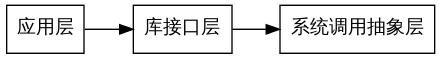
\includegraphics{./figures/0-overview.jpg}
\caption{kmod-11 项目系统结构层次图}
\end{figure}

下面按照这样的三层架构,按照应用层,库接口层,抽象层的顺序,依次分析。

\subsubsection{应用层}

应用层实现了6个常用的用户命令,分别是 insmod, rmmod, lsmod, modinfo,
depmod, modprobe.

\begin{figure}[htbp]
\centering
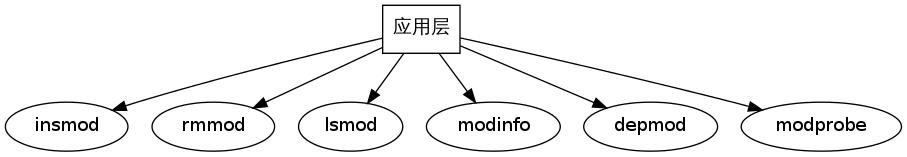
\includegraphics{./figures/1-app.jpg}
\caption{kmod-11 项目应用层结构图}
\end{figure}

\paragraph{insmod 命令}

该命令的功能是: 向Linux内核中插入一个模块

{\begin{shaded}\begin{verbatim}
$ ./kmod-11/tools/insmod -h

Usage:
    insmod [options] filename [args]
Options:
    -V, --version     show version
    -h, --help        show this help
\end{verbatim}\end{shaded}}
\paragraph{rmmod 命令}

该命令的功能是: 删除内核中的模块

{\begin{shaded}\begin{verbatim}
$ ./kmod-11/tools/rmmod -h
Usage:
    rmmod [options] modulename ...
Options:
    -f, --force       forces a module unload and may crash your
                  machine. This requires Forced Module Removal
                  option in your kernel. DANGEROUS
    -s, --syslog      print to syslog, not stderr
    -v, --verbose     enables more messages
    -V, --version     show version
    -h, --help        show this help
\end{verbatim}\end{shaded}}
\paragraph{lsmod 命令}

该命令的功能是: 列出内核已载入模块的状态

{\begin{shaded}\begin{verbatim}
$ ./kmod-11/tools/lsmod -h
Usage: ./kmod-11/tools/lsmod
\end{verbatim}\end{shaded}}
\paragraph{modinfo 命令}

该命令的功能是: 显示内核模块的信息

{\begin{shaded}\begin{verbatim}
$ ./kmod-11/tools/modinfo -h
Usage:
    modinfo [options] filename [args]
Options:
    -a, --author                Print only 'author'
    -d, --description           Print only 'description'
    -l, --license               Print only 'license'
    -p, --parameters            Print only 'parm'
    -n, --filename              Print only 'filename'
    -0, --null                  Use \0 instead of \n
    -F, --field=FIELD           Print only provided FIELD
    -k, --set-version=VERSION   Use VERSION instead of `uname -r`
    -b, --basedir=DIR           Use DIR as filesystem root for /lib/modules
    -V, --version               Show version
    -h, --help                  Show this help
$ 
\end{verbatim}\end{shaded}}
\paragraph{depmod 命令}

该命令的功能是: 分析可加载模块的依赖性,生成modules.dep文件和映射文件。

{\begin{shaded}\begin{verbatim}
$ ./kmod-11/tools/depmod -h
Usage:
    depmod -[aA] [options] [forced_version]

If no arguments (except options) are given, "depmod -a" is assumed

depmod will output a dependency list suitable for the modprobe utility.

Options:
    -a, --all            Probe all modules
    -A, --quick          Only does the work if there's a new module
    -e, --errsyms        Report not supplied symbols
    -n, --show           Write the dependency file on stdout only
    -P, --symbol-prefix  Architecture symbol prefix
    -C, --config=PATH    Read configuration from PATH
    -v, --verbose        Enable verbose mode
    -w, --warn           Warn on duplicates
    -V, --version        show version
    -h, --help           show this help

The following options are useful for people managing distributions:
    -b, --basedir=DIR    Use an image of a module tree.
    -F, --filesyms=FILE  Use the file instead of the
                     current kernel symbols.
    -E, --symvers=FILE   Use Module.symvers file to check
                     symbol versions.
$ 
\end{verbatim}\end{shaded}}
\paragraph{modprobe 命令}

该命令的功能是: Linux内核添加或者删除模块

{\begin{shaded}\begin{verbatim}
$ ./kmod-11/tools/modprobe -h
Usage:
    modprobe [options] [-i] [-b] modulename
    modprobe [options] -a [-i] [-b] modulename [modulename...]
    modprobe [options] -r [-i] modulename
    modprobe [options] -r -a [-i] modulename [modulename...]
    modprobe [options] -c
    modprobe [options] --dump-modversions filename
Management Options:
    -a, --all                   Consider every non-argument to
                            be a module name to be inserted
                            or removed (-r)
    -r, --remove                Remove modules instead of inserting
        --remove-dependencies   Also remove modules depending on it
    -R, --resolve-alias         Only lookup and print alias and exit
        --first-time            Fail if module already inserted or removed
    -i, --ignore-install        Ignore install commands
    -i, --ignore-remove         Ignore remove commands
    -b, --use-blacklist         Apply blacklist to resolved alias.
    -f, --force                 Force module insertion or removal.
                            implies --force-modversions and
                            --force-vermagic
        --force-modversion      Ignore module's version
        --force-vermagic        Ignore module's version magic

Query Options:
    -D, --show-depends          Only print module dependencies and exit
    -c, --showconfig            Print out known configuration and exit
    -c, --show-config           Same as --showconfig
        --show-modversions      Dump module symbol version and exit
        --dump-modversions      Same as --show-modversions

General Options:
    -n, --dry-run               Do not execute operations, just print out
    -n, --show                  Same as --dry-run
    -C, --config=FILE           Use FILE instead of default search paths
    -d, --dirname=DIR           Use DIR as filesystem root for /lib/modules
    -S, --set-version=VERSION   Use VERSION instead of `uname -r`
    -s, --syslog                print to syslog, not stderr
    -q, --quiet                 disable messages
    -v, --verbose               enables more messages
    -V, --version               show version
    -h, --help                  show this help
$ 
\end{verbatim}\end{shaded}}
\subsubsection{库接口层}

库接口层包含了 libkmod 目录下的形如 libkmod-xxx.c
的模块文件,其中涉及用到的编程接口将近100个,形如 kmod\_xxx\_xxx\_xxx
的接口函数。

按照这些接口函数的归属模块划分,我们经过代码分析,可以将它们分为6个重要的核心子模块,分别是
kmod\_ctx, kmod\_module, kmod\_config, kmod\_list, kmod\_elf,
kmod\_file。

\begin{figure}[htbp]
\centering
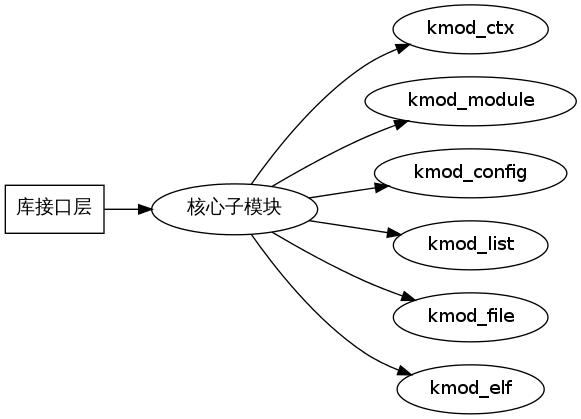
\includegraphics{./figures/2-core.jpg}
\caption{kmod-11 项目库接口层核心子模块结构图}
\end{figure}

另外还有6个属于基础类的子模块,为以上6个核心子模块提供支持,分别是 hash,
index\_mm,elf,list,array,log。

\begin{figure}[htbp]
\centering
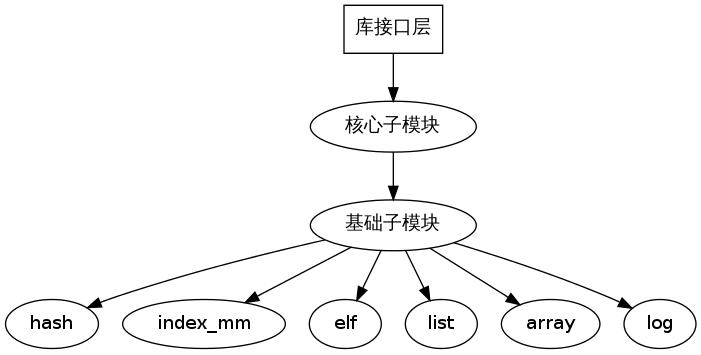
\includegraphics{./figures/2-base.jpg}
\caption{kmod-11 项目库接口层基础子模块结构图}
\end{figure}

以下在模块分析小节将分别对这12个模块进行详细说明。

\subsubsection{系统调用抽象层}

系统调用抽象层的实现代码主要集中在 testsuite
目录下,其中最重要的2个实现包含 init\_module 系统调用和 delete\_module
系统调用的模拟实现。

\begin{figure}[htbp]
\centering
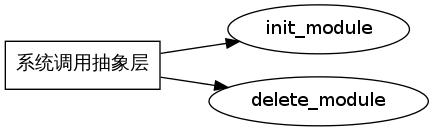
\includegraphics{./figures/3-syscall.jpg}
\caption{kmod-11 项目系统调用抽象层结构图}
\end{figure}

\subsubsection{各层之间相互关系图}

以上的命令,库,核心子模块,基础子模块以及系统调用抽象层,之间的关系并不是明显分开的,而是互相之间有交错的关系。为了更清楚的说明整个系统各个层次之间的调用关系,我们以下图为例,做简要说明。

\begin{figure}[htbp]
\centering
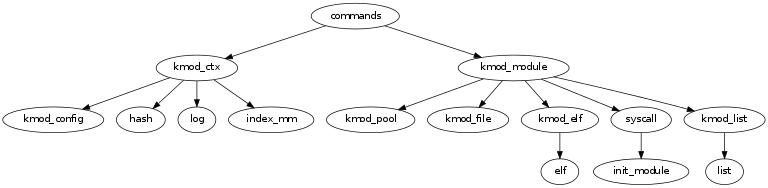
\includegraphics{./figures/sys.jpg}
\caption{kmod-11 项目系统各层结构关系图}
\end{figure}

其中命令层就是应用层,一般命令的实现都会首先使用 kmod\_ctx 和
kmod\_module 两个核心子模块的接口,其中 kmod\_ctx 调用了 kmod\_config
核心子模块和 hash, log, index\_mm 基础子模块的接口功能,kmod\_module
调用了 kmod\_file, kmod\_elf, kmod\_list
这3个核心子模块的接口功能,以及简介调用了 elf, list
这2个基础子模块的接口功能,同时还使用了模拟层中有关系统调用模拟实现的接口。

因此在我们所列出的6个核心子模块中,kmod\_ctx 和 kmod\_module
这2个核心子模块占据着更为重要的作用,是整个 libkmod
库的核心中的核心。在下面的分析中,我们还会详细论述它们的功能。

\subsection{2. 模块分析}

\subsubsection{kmod\_ctx}

\subsubsection{kmod\_module}

\subsubsection{kmod\_elf}

\subsubsection{kmod\_file}

\subsubsection{kmod\_config}

\subsubsection{hash}

\subsubsection{kmod\_list}

\subsubsection{index\_mm}

\subsubsection{elf}

\subsubsection{list}

\subsubsection{array}

\subsubsection{log}

\subsection{3. 运行时调试图}

\subsubsection{insmod 命令运行时调试图}

\paragraph{编写测试用内核模块源码 hello.c}

{\begin{shaded}\begin{verbatim}
$ cat hello.c 

#include <linux/module.h>
#include <linux/kernel.h>

MODULE_AUTHOR("AKAEDU");
MODULE_DESCRIPTION("module example ");
MODULE_LICENSE("GPL");

int global = 100;

int __init 
akae_init (void)
{
    int local = 200;
    printk ("Hello, akaedu\n");

    printk(".text = %p\n", akae_init);
    printk(".data = %p\n", &global);
    printk(".stack = %p\n", &local);
    return 0;
}

void __exit
akae_exit (void)
{
    int local = 300;
    printk ("module exit\n");

    printk(".text = %p\n", akae_exit);
    printk(".data = %p\n", &global);
    printk(".stack = %p\n", &local);
    return ;
}

module_init(akae_init);
module_exit(akae_exit);
$ 
\end{verbatim}\end{shaded}}
\paragraph{编写测试用内核模块的 Makefile 文件 Makefile}

{\begin{shaded}\begin{verbatim}
$ cat Makefile 

obj-m := hello.o

KDIR := /usr/src/linux-headers-3.2.0-29-generic-pae/

all:
    make -C $(KDIR) SUBDIRS=$(PWD)  modules

clean:
    rm -rf *.o *.ko *.mod.* *.cmd 
    rm -rf .*

$ 
\end{verbatim}\end{shaded}}
\paragraph{编译内核模块 hello.ko}

{\begin{shaded}\begin{verbatim}
$ cd hello-module/ 
$ make
make -C /usr/src/linux-headers-3.2.0-29-generic-pae/    SUBDIRS=/home/akaedu/Github/comment-subs/hello-module   modules
make[1]: Entering directory `/usr/src/linux-headers-3.2.0-29-generic-pae'
  CC [M]  /home/akaedu/Github/comment-subs/hello-module/hello.o
  Building modules, stage 2.
  MODPOST 1 modules
  CC      /home/akaedu/Github/comment-subs/hello-module/hello.mod.o
  LD [M]  /home/akaedu/Github/comment-subs/hello-module/hello.ko
make[1]: Leaving directory `/usr/src/linux-headers-3.2.0-29-generic-pae'
$ 
\end{verbatim}\end{shaded}}
\paragraph{编译生成测试用工具 insmod}

{\begin{shaded}\begin{verbatim}
$ cd kmod-11/ 
$ make
make --no-print-directory all-recursive
Making all in .
  CC       libkmod/libkmod.lo
  CC       libkmod/libkmod-list.lo
  CC       libkmod/libkmod-config.lo
  CC       libkmod/libkmod-index.lo
  CC       libkmod/libkmod-module.lo
  CC       libkmod/libkmod-file.lo
  CC       libkmod/libkmod-elf.lo
  CC       libkmod/libkmod-hash.lo
  CC       libkmod/libkmod-array.lo
  CC       libkmod/libkmod-util.lo
  CCLD     libkmod/libkmod-util.la
  CCLD     libkmod/libkmod.la
  CCLD     libkmod/libkmod-private.la
  CC       tools/kmod.o
  CC       tools/lsmod.o
  CC       tools/rmmod.o
  CC       tools/insmod.o
  CC       tools/modinfo.o
  CC       tools/modprobe.o
  CC       tools/depmod.o
  CC       tools/log.o
  CCLD     tools/kmod
  CCLD     tools/kmod-nolib
  GEN      libkmod/libkmod.pc
Making all in libkmod/docs
make[2]: Nothing to be done for `all'.
Making all in man
  GEN      depmod.d.5
  GEN      modprobe.d.5
  GEN      modules.dep.5
  GEN      depmod.8
  GEN      insmod.8
  GEN      lsmod.8
  GEN      rmmod.8
  GEN      modprobe.8
  GEN      modinfo.8
$ 
\end{verbatim}\end{shaded}}
\paragraph{使用测试用工具 insmod 插入内核模块}

{\begin{shaded}\begin{verbatim}
$ sudo ./kmod-11/tools/insmod hello-module/hello.ko 
\end{verbatim}\end{shaded}}
\paragraph{查看插入内核模块后的打印结果}

{\begin{shaded}\begin{verbatim}
$ lsmod | grep hello
hello                  12415  0 
$ dmesg | tail
[350775.859640] usb 2-2.1: USB disconnect, device number 14
[350777.611134] Bluetooth: hci0 urb c7304180 submission failed
[350778.217886] usb 2-2.1: new full-speed USB device number 15 using uhci_hcd
[352048.604051] usb 2-2.1: USB disconnect, device number 15
[352048.630829] Bluetooth: hci0 urb dd3d3000 submission failed
[352049.254135] usb 2-2.1: new full-speed USB device number 16 using uhci_hcd
[352111.505217] Hello, akaedu
[352111.505223] .text = e0844000
[352111.505225] .data = e0c03000
[352111.505227] .stack = df6e3f54
$ 
\end{verbatim}\end{shaded}}
\paragraph{重复插入同样的内核模块系统会报错}

{\begin{shaded}\begin{verbatim}
$ sudo ./kmod-11/tools/insmod hello-module/hello.ko 
insmod: ERROR: could not insert module hello-module/hello.ko: File exists
$ lsmod | grep hello
hello                  12415  0 
\end{verbatim}\end{shaded}}
\subsubsection{rmmod 命令运行时调试图}

\paragraph{使用测试用工具 rmmod 卸载内核模块}

{\begin{shaded}\begin{verbatim}
$ sudo ./kmod-11/tools/rmmod hello-module/hello.ko
$ (rmmod 命令的执行,运行在 hello 的后面加上 .ko 的后缀,这个和以前的命令有所不同)
\end{verbatim}\end{shaded}}
\paragraph{查看卸载内核模块后的打印结果}

{\begin{shaded}\begin{verbatim}
$ lsmod | grep hello
$ (可以看到上面命令的执行结果没有任何输出信息)
$ dmesg | tail
[352048.630829] Bluetooth: hci0 urb dd3d3000 submission failed
[352049.254135] usb 2-2.1: new full-speed USB device number 16 using uhci_hcd
[352111.505217] Hello, akaedu
[352111.505223] .text = e0844000
[352111.505225] .data = e0c03000
[352111.505227] .stack = df6e3f54
[352365.795618] module exit
[352365.795624] .text = e0c01000
[352365.795626] .data = e0c03000
[352365.795628] .stack = dd197f40
$ 
\end{verbatim}\end{shaded}}
\subsection{4. 运行流程分析}

\subsubsection{insmod 命令实现流程}

insmod 命令和其他所有命令一样,都是采用了一个统一的调用方法。实现了一个
struct kmod\_cmd 的数据结构,这个数据结构定义在 kmod-11/tools/kmod.h
文件中。

{\begin{shaded}\begin{verbatim}
struct kmod_cmd {
    const char *name;
    int (*cmd)(int argc, char *argv[]);
    const char *help;
};
\end{verbatim}\end{shaded}}
在 kmod-11/tools/insmod.c 文件中,用这个结构体定义了

{\begin{shaded}\begin{verbatim}
160 
161 const struct kmod_cmd kmod_cmd_compat_insmod = {
162         .name = "insmod",
163         .cmd = do_insmod,
164         .help = "compat insmod command",
165 };
\end{verbatim}\end{shaded}}
在 kmod-11/tools/kmod.c 文件中,实现了一个通用的 main 方法。

{\begin{shaded}\begin{verbatim}
166 int main(int argc, char *argv[])
167 {
168         int err;
169 
170         if (strcmp(program_invocation_short_name, "kmod") == 0)
171                 err = handle_kmod_commands(argc, argv);
172         else
173                 err = handle_kmod_compat_commands(argc, argv);
174 
175         return err;
176 }
\end{verbatim}\end{shaded}}
在这个main函数中,调用了 handle\_kmod\_compat\_commands 函数。

{\begin{shaded}\begin{verbatim}
149 
150 static int handle_kmod_compat_commands(int argc, char *argv[])
151 {
152         const char *cmd;
153         size_t i;
154 
155         cmd = basename(argv[0]);
156 
157         for (i = 0; i < ARRAY_SIZE(kmod_compat_cmds); i++) {
158                 if (strcmp(kmod_compat_cmds[i]->name, cmd) == 0)
159                         return kmod_compat_cmds[i]->cmd(argc, argv);
160         }
161 
162         return -ENOENT;
163 }
164 
\end{verbatim}\end{shaded}}
handle\_kmod\_compat\_commands 这个函数很简单,就是一个for循环遍历整个
kmod\_compat\_cmds,找出每一个 kmod\_compat\_cmds{[}i{]} 来进行名称 name
匹配,如果匹配上了,就调用相应的函数指针 cmd 来执行该操作。

kmod\_compat\_cmds 这个数组目前有6个元素,分别就是在 insmod.c rmmod.c
lsmod.c modinfo.c depmod.c modprobe.c 这6个文件中定义的全局结构体。

{\begin{shaded}\begin{verbatim}
 44
 45 static const struct kmod_cmd *kmod_compat_cmds[] = {
 46         &kmod_cmd_compat_lsmod,
 47         &kmod_cmd_compat_rmmod,
 48         &kmod_cmd_compat_insmod,
 49         &kmod_cmd_compat_modinfo,
 50         &kmod_cmd_compat_modprobe,
 51         &kmod_cmd_compat_depmod,
 52 };
\end{verbatim}\end{shaded}}
最后所有 tools
目录下的可执行文件,都是以软链接的方式,链接到唯一的一个可执行文件
kmod-nolib 上。

{\begin{shaded}\begin{verbatim}
$ ls kmod-11/tools/ -l | grep ^l
lrwxrwxrwx 1 akaedu akaedu     10 Jun  9 19:23 depmod -> kmod-nolib
lrwxrwxrwx 1 akaedu akaedu     10 Jun  9 19:23 insmod -> kmod-nolib
lrwxrwxrwx 1 akaedu akaedu     10 Jun  9 19:23 lsmod -> kmod-nolib
lrwxrwxrwx 1 akaedu akaedu     10 Jun  9 19:23 modinfo -> kmod-nolib
lrwxrwxrwx 1 akaedu akaedu     10 Jun  9 19:23 modprobe -> kmod-nolib
lrwxrwxrwx 1 akaedu akaedu     10 Jun  9 19:23 rmmod -> kmod-nolib
$ 
\end{verbatim}\end{shaded}}
我们可以用一张图来表示这些文件和数据结构之间的关系。

\begin{figure}[htbp]
\centering
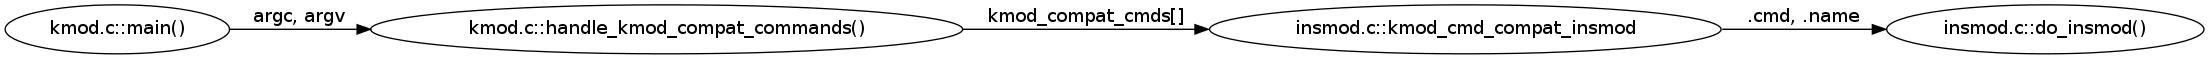
\includegraphics{./figures/cmd.jpg}
\caption{命令实现结构图}
\end{figure}

\textbf{do\_insmod 核心代码分析}

分析到这里,我们就进入到了 insmod 命令实现最核心的部分 do\_insmod()
函数,后面的其他几个命令也都是类似的方法,进入到 do\_xxx()
中,之后的分析关于这部分不再赘述。下面我们来看看 do\_insmod()
函数实现中最核心的部分代码摘要。

{\begin{shaded}\begin{verbatim}
do_insmod()
{
    opts = argv[x]; // name=value
    ctx = kmod_new(NULL, &null_config);
    err = kmod_module_new_from_path(ctx, filename, &mod);
    err = kmod_module_insert_module(mod, 0, opts);
    kmod_module_unref(mod);
    kmod_unref(ctx);
}
\end{verbatim}\end{shaded}}
注意这个小节中后面的绝大部分代码都不是原代码的引用,而是将其中最核心的函数调用和传入传出的参数整理到函数体内部,为便于查看函数调用关系而做了简化。

\begin{figure}[htbp]
\centering
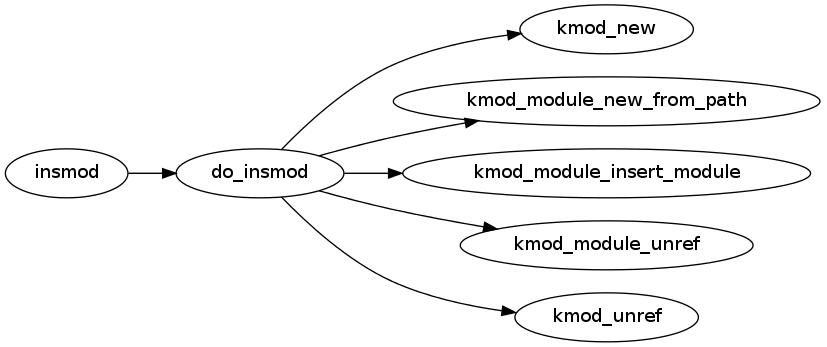
\includegraphics{./figures/insmod.jpg}
\caption{insmod 调用层次图}
\end{figure}

do\_insmod() 的实现可以分为5个步骤

\begin{itemize}
\item
  创建模块的上下文 struct kmod\_ctx ctx
\item
  通过 filename 和 ctx 获得模块 struct kmod\_module mod
\item
  将 mod 插入到当前模块列表中, 完成真正的插入内核功能
\item
  释放 mod
\item
  释放 ctx
\end{itemize}
涉及到两个模块的5个接口,两个模块是

\begin{itemize}
\item
  libkmod/libkmod.c
  \begin{itemize}
  \item
    kmod\_new()
  \item
    kmod\_unref()
  \end{itemize}
\item
  libkmod/libkmod-module.c
  \begin{itemize}
  \item
    kmod\_module\_new\_from\_path()
  \item
    kmod\_module\_insert\_module()
  \item
    kmod\_module\_unref()
  \end{itemize}
\end{itemize}
\subsubsection{rmmod 命令实现流程}

\textbf{do\_rmmod 核心代码分析}

下面我们来看看 do\_rmmod() 函数实现中最核心的部分代码摘要。

{\begin{shaded}\begin{verbatim}
do_rmmod()
{
    log_open(use_syslog);
    ctx = kmod_new(NULL, &null_config);
    log_setup_kmod_log(ctx, verbose);
    arg = argv[i];
    err = kmod_module_new_from_path(ctx, arg, &mod);
    err = kmod_module_new_from_name(ctx, arg, &mod);
    check_module_inuse(mod);
    err = kmod_module_remove_module(mod, flags);
    kmod_module_unref(mod);
    kmod_unref(ctx);
    log_close();
}
\end{verbatim}\end{shaded}}
\begin{figure}[htbp]
\centering
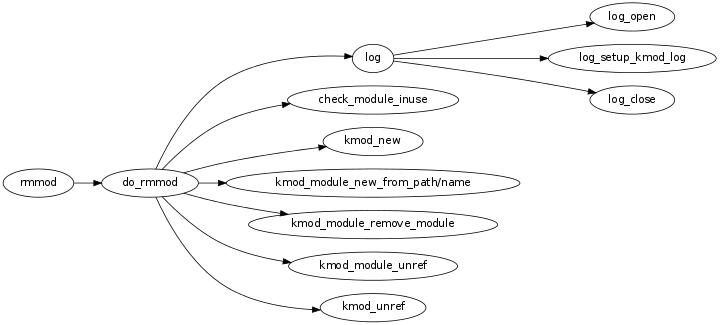
\includegraphics{./figures/rmmod.jpg}
\caption{rmmod 调用层次图}
\end{figure}

do\_rmmod() 的实现可以分为5个步骤

\begin{itemize}
\item
  创建模块的上下文 struct kmod\_ctx ctx
\item
  通过 filename 和 ctx 获得模块 struct kmod\_module mod
\item
  将 mod 插入到当前模块列表中, 完成真正的插入内核功能
\item
  释放 mod
\item
  释放 ctx
\end{itemize}
涉及到两个模块的5个接口,两个模块是

\begin{itemize}
\item
  libkmod/libkmod.c
  \begin{itemize}
  \item
    kmod\_new()
  \item
    kmod\_unref()
  \end{itemize}
\item
  libkmod/libkmod-module.c
  \begin{itemize}
  \item
    kmod\_module\_new\_from\_path()
  \item
    kmod\_module\_insert\_module()
  \item
    kmod\_module\_unref()
  \end{itemize}
\end{itemize}
\subsubsection{lsmod 命令实现流程}

\begin{figure}[htbp]
\centering
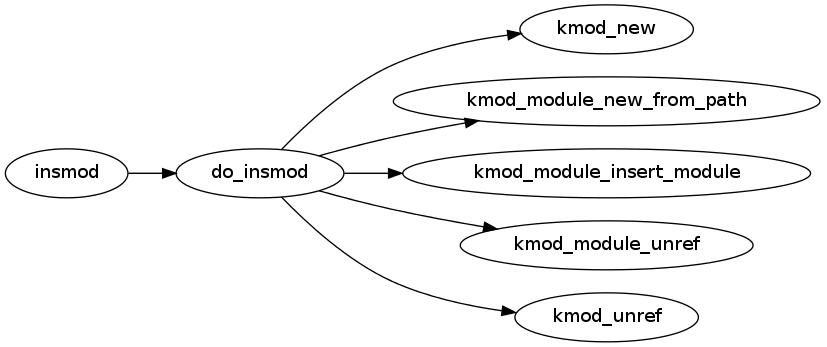
\includegraphics{./figures/insmod.jpg}
\caption{insmod 调用层次图}
\end{figure}

\subsubsection{modinfo 命令实现流程}

\begin{figure}[htbp]
\centering
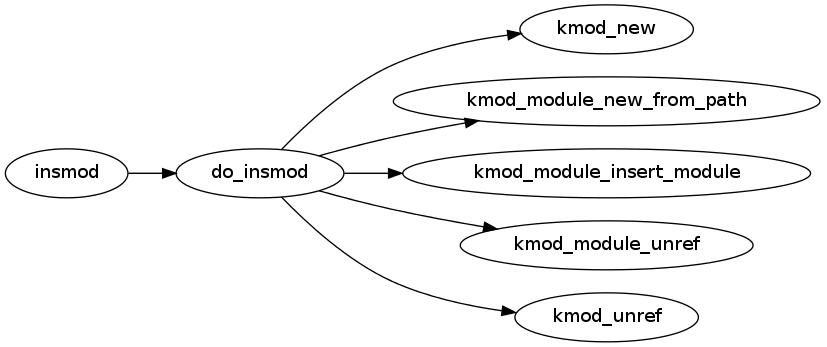
\includegraphics{./figures/insmod.jpg}
\caption{insmod 调用层次图}
\end{figure}

\subsubsection{depmod 命令实现流程}

\begin{figure}[htbp]
\centering
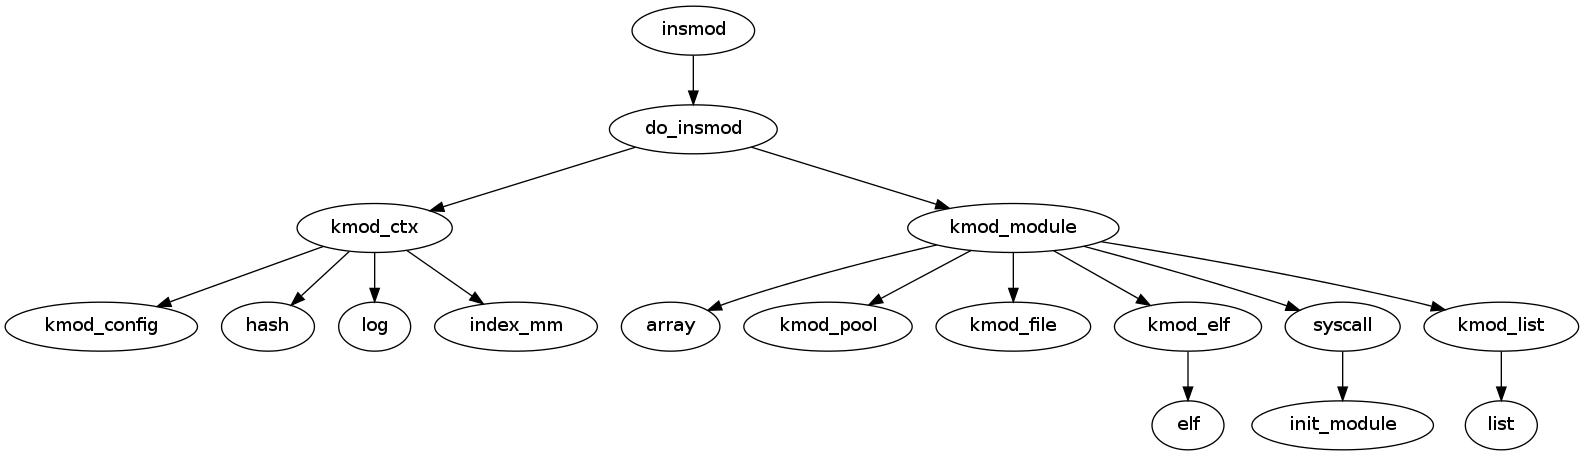
\includegraphics{./figures/depmod.jpg}
\caption{depmod 调用层次图}
\end{figure}

\textbf{do\_depmod() 核心代码分析}

{\begin{shaded}\begin{verbatim}
do_depmod(int argc, char *argv[])
{
    out = stdout;       
    ctx = kmod_new(cfg.dirname, &null_kmod_config);

    err = depmod_init(&depmod, &cfg, ctx);
    err = depmod_load_symvers(&depmod, module_symvers);
    err = depmod_load_system_map(&depmod, system_map);
    err = cfg_load(&cfg, config_paths);
    err = depmod_modules_search(&depmod);
    err = kmod_module_new_from_path(depmod.ctx, path, &mod);
    err = depmod_module_add(&depmod, mod);
    err = depmod_modules_build_array(&depmod);
    depmod_modules_sort(&depmod);
    err = depmod_load(&depmod);

    err = depmod_output(&depmod, out);
    depmod_shutdown(&depmod);
    cfg_free(&cfg);
    kmod_unref(ctx);
}
\end{verbatim}\end{shaded}}
下面根据这个核心代码,将在一层逻辑过程中调用到的函数,做一个简要的说明。
所有这些函数可以分为3类,分别形如 kmod\_xxx,depmod\_xxx, cfg\_xxx
开头的。

\textbf{kmod\_xxx} 包含 kmod\_new, kmod\_module\_new\_from\_path,
kmod\_unref 这3个在之前的代码分析中介绍过。

\textbf{depmod\_xxx} 这些函数都被声明为 static 的类型,说明仅仅只是为
depmod 命令的实现而服务的,不属于 libkmod 库要提供的接口。 * depmod
内部子模块上层接口 - depmod\_init - depmod\_load\_symvers -
depmod\_load\_system\_map - depmod\_modules\_search -
depmod\_module\_add - depmod\_modules\_build\_array -
depmod\_modules\_sort - depmod\_shutdown

\begin{itemize}
\item
  围绕上面这些函数,还需要调用到如下接口

  static int depmod\_init(struct depmod *depmod, struct cfg *cfg, struct
  kmod\_ctx *ctx) \{ array\_init(\&depmod-\textgreater{}modules, 128);

{\begin{shaded}\begin{verbatim}
depmod->modules_by_uncrelpath = hash_new(512, NULL);
depmod->modules_by_name = hash_new(512, NULL);
depmod->symbols = hash_new(2048, (void (*)(void *))symbol_free);

hash_free(depmod->modules_by_name);
hash_free(depmod->modules_by_uncrelpath);

return err;
\end{verbatim}\end{shaded}}
  \}

  static int depmod\_load\_symvers(struct depmod *depmod, const char
  *filename) \{ fp = fopen(filename, ``r''); while (fgets(line,
  sizeof(line), fp) != NULL) \{ ver = strtok(line, " \t");

{\begin{shaded}\begin{verbatim}
depmod_symbol_add(depmod, sym, crc, NULL);
depmod_add_fake_syms(depmod);

fclose(fp);
return 0;
\end{verbatim}\end{shaded}}
  \}

  static int depmod\_load\_system\_map(struct depmod *depmod, const char
  *filename) \{ fp = fopen(filename, ``r''); while (fgets(line,
  sizeof(line), fp) != NULL) \{ p = strchr(line, ' ');
  depmod\_symbol\_add(depmod, p + ksymstr\_len, 0, NULL);
  depmod\_add\_fake\_syms(depmod); fclose(fp); return 0; \}

  static int depmod\_modules\_search(struct depmod *depmod) \{ DIR *d =
  opendir(depmod-\textgreater{}cfg-\textgreater{}dirname); err =
  depmod\_modules\_search\_dir(depmod, d, baselen, path); closedir(d);
  return err; \}

  static int depmod\_module\_add(struct depmod *depmod, struct
  kmod\_module *kmod) \{ modname = kmod\_module\_get\_name(kmod);

{\begin{shaded}\begin{verbatim}
mod = calloc(1, sizeof(struct mod) + modnamelen);

array_init(&mod->deps, 4);

err = hash_add_unique(depmod->modules_by_name, mod->modname, mod);

return 0;
\end{verbatim}\end{shaded}}
  \}

  static int depmod\_modules\_build\_array(struct depmod *depmod) \{
  hash\_iter\_init(depmod-\textgreater{}modules\_by\_name,
  \&module\_iter);

{\begin{shaded}\begin{verbatim}
while (hash_iter_next(&module_iter, NULL, &v)) {
        struct mod *mod = (struct mod *) v;
        mod->idx = depmod->modules.count;
        err = array_append(&depmod->modules, mod);
        if (err < 0)
                return err;
}
return 0;
\end{verbatim}\end{shaded}}
  \}

  static void depmod\_modules\_sort(struct depmod *depmod) \{
  snprintf(order\_file, sizeof(order\_file), ``\%s/modules.order'',
  depmod-\textgreater{}cfg-\textgreater{}dirname); fp =
  fopen(order\_file, ``r'');

{\begin{shaded}\begin{verbatim}
while (fgets(line, sizeof(line), fp) != NULL) {
    mod = hash_find(depmod->modules_by_uncrelpath, line);
}

array_sort(&depmod->modules, mod_cmp);

for (idx = 0; idx < depmod->modules.count; idx++) {
        struct mod *m = depmod->modules.array[idx];
        m->idx = idx;
}
\end{verbatim}\end{shaded}}
  \}

  static void depmod\_shutdown(struct depmod *depmod) \{
  hash\_free(depmod-\textgreater{}symbols);

{\begin{shaded}\begin{verbatim}
hash_free(depmod->modules_by_uncrelpath);

hash_free(depmod->modules_by_name);

for (i = 0; i < depmod->modules.count; i++)
        mod_free(depmod->modules.array[i]);

array_free_array(&depmod->modules);

kmod_unref(depmod->ctx);
\end{verbatim}\end{shaded}}
  \}
\end{itemize}
\textbf{cfg\_xxx}

{\begin{shaded}\begin{verbatim}
static int cfg_load(struct cfg *cfg, const char * const *cfg_paths)
{
    for (i = 0; cfg_paths[i] != NULL; i++)
            cfg_files_list(&files, &n_files, cfg_paths[i]);

    for (i = 0; i < n_files; i++) {
            struct cfg_file *f = files[i];
            cfg_file_parse(cfg, f->path);
            cfg_file_free(f);
    }
    free(files);

    if (cfg->searches == NULL)
            cfg_search_add(cfg, "updates", 0);

    return 0;
}

static void cfg_free(struct cfg *cfg)
{
    while (cfg->overrides) {
            struct cfg_override *tmp = cfg->overrides;
            cfg->overrides = cfg->overrides->next;
            cfg_override_free(tmp);
    }

    while (cfg->searches) {
            struct cfg_search *tmp = cfg->searches;
            cfg->searches = cfg->searches->next;
            cfg_search_free(tmp);
    }
}
\end{verbatim}\end{shaded}}
在 depmod.c 文件的实现中,depmod\_output 负责最后各类文件的输出功能。

{\begin{shaded}\begin{verbatim}
2161 static int depmod_output(struct depmod *depmod, FILE *out)
2162 {
2163         static const struct depfile {
2164                 const char *name;
2165                 int (*cb)(struct depmod *depmod, FILE *out);
2166         } *itr, depfiles[] = {
2167                 { "modules.dep", output_deps },
2168                 { "modules.dep.bin", output_deps_bin },
2169                 { "modules.alias", output_aliases },
2170                 { "modules.alias.bin", output_aliases_bin },
2171                 { "modules.softdep", output_softdeps },
2172                 { "modules.symbols", output_symbols },
2173                 { "modules.symbols.bin", output_symbols_bin },
2174                 { "modules.builtin.bin", output_builtin_bin },
2175                 { "modules.devname", output_devname },
2176                 { }
2177         };
\end{verbatim}\end{shaded}}
其中输出到 /lib/modules/3.2.0-29-generic-pae/modules.dep
文件的输出函数是 output\_deps 通过修改如下 fprintf(out, \ldots{})
函数,增添输出到标准输出 stdout 的 fprintf(stdout, \ldots{})
则可以在屏幕上看到运行 depmod 命令时候的全部输出结果,这个结果和
modules.dep 文件中的内容是完全一样的。

{\begin{shaded}\begin{verbatim}
1790 static int output_deps(struct depmod *depmod, FILE *out)
1791 {
1792         size_t i;
1793 
1794         for (i = 0; i < depmod->modules.count; i++) {
1795                 const struct mod **deps, *mod = depmod->modules.array[i];
...
1804                 fprintf(out, "%s:", p);
1805                 fprintf(stdout, "%s:", p);
...
1824                         fprintf(out, " %s", mod_get_compressed_path(d));
1825                         fprintf(stdout, " %s", mod_get_compressed_path(d));
...
1828         end:
1829                 putc('\n', out);
1830                 putc('\n', stdout);
... 
1834 }
\end{verbatim}\end{shaded}}
\subsubsection{modprobe 命令实现流程}

\textbf{do\_modprobe() 核心代码分析}

{\begin{shaded}\begin{verbatim}
do_modprobe(int argc, char *argv[])
{
    log_open(use_syslog);

    snprintf(dirname_buf, sizeof(dirname_buf), "%s/lib/modules/%s", root, kversion);
    dirname = dirname_buf;

    ctx = kmod_new(dirname, config_paths);

    log_setup_kmod_log(ctx, verbose);
    kmod_load_resources(ctx);

    if (do_xxx)
        err = show_config(ctx); 
        err = show_modversions(ctx, args[0]);
        err = insmod_all(ctx, args, nargs);
        err = rmmod_all(ctx, args, nargs); 

    err = options_from_array(args, nargs, &opts);
    err = insmod(ctx, args[0], opts);

    kmod_unref(ctx);

    log_close();
}
\end{verbatim}\end{shaded}}
\paragraph{insmod\_all}

{\begin{shaded}\begin{verbatim}
static int insmod_all(struct kmod_ctx *ctx, char **args, int nargs)
{
        for (i = 0; i < nargs; i++) 
        err = insmod(ctx, args[i], NULL);

    return err;
}
\end{verbatim}\end{shaded}}
\paragraph{insmod}

{\begin{shaded}\begin{verbatim}
-> kmod_module_probe_insert_module()
\end{verbatim}\end{shaded}}
\paragraph{kmod\_module\_probe\_insert\_module}

{\begin{shaded}\begin{verbatim}
int kmod_module_probe_insert_module(mod, flags, extra_options, run_install)
{
    err = kmod_module_get_probe_list(mod, !!(flags & KMOD_PROBE_IGNORE_COMMAND), &list);

    kmod_list_foreach(l, list) 
    {
        struct kmod_module *m = l->data;
        err = kmod_module_insert_module(m, flags, options);
    }
}

-> kmod_module_get_probe_list
    -> __kmod_module_get_probe_list
        -> __kmod_module_get_probe_list
            -> kmod_module_get_dependencies
                ->  module_get_dependencies_noref
                    -> kmod_module_parse_depline
\end{verbatim}\end{shaded}}
\paragraph{kmod\_module\_get\_dependencies}

{\begin{shaded}\begin{verbatim}
kmod_list *kmod_module_get_dependencies(struct kmod_module *mod)
{
    module_get_dependencies_noref(mod);

    kmod_list_foreach(l, mod->dep)
    {
        l_new = kmod_list_append(list_new, kmod_module_ref(l->data));
        list_new = l_new;
    }

    return list_new;
}
\end{verbatim}\end{shaded}}
\paragraph{module\_get\_dependencies\_noref}

{\begin{shaded}\begin{verbatim}
kmod_list *module_get_dependencies_noref(struct kmod_module *mod)
{
    char *line = kmod_search_moddep(mod->ctx, mod->name);

    kmod_module_parse_depline(mod, line);

    return mod->dep;
}
\end{verbatim}\end{shaded}}
\paragraph{kmod\_search\_moddep}

{\begin{shaded}\begin{verbatim}
char *kmod_search_moddep(struct kmod_ctx *ctx, const char *name)
{
    // name = nfs;      // modprobe nfs
    return index_mm_search(ctx->indexes[KMOD_INDEX_MODULES_DEP], name);

    DBG(ctx, "file=%s modname=%s\n", fn, name);

    idx = index_file_open(fn);
    line = index_search(idx, name);
    index_file_close(idx);

    return line;
}
\end{verbatim}\end{shaded}}
\paragraph{kmod\_module\_parse\_depline}

{\begin{shaded}\begin{verbatim}
int kmod_module_parse_depline(struct kmod_module *mod, char *line)
{
    for (p = strtok_r(p, " \t", &saveptr); p != NULL;
         p = strtok_r(NULL, " \t", &saveptr)) 
    {
        err = kmod_module_new_from_path(ctx, path, &depmod);
        list = kmod_list_prepend(list, depmod);
        n++;
    }

    mod->dep = list;
    mod->n_dep = n;

    return n;
}
\end{verbatim}\end{shaded}}
\subsection{5. 函数接口分析}

\subsubsection{kmod\_new() 核心代码分析}

{\begin{shaded}\begin{verbatim}
kmod_ctx *kmod_new(char *dirname, char *config_paths)
{
    ctx = calloc(1, sizeof(struct kmod_ctx));
    ctx->dirname = get_kernel_release(dirname);
    err = kmod_config_new(ctx, &ctx->config, config_paths);
    ctx->modules_by_name = hash_new(KMOD_HASH_SIZE, NULL);

    return ctx;
}
\end{verbatim}\end{shaded}}
\begin{figure}[htbp]
\centering
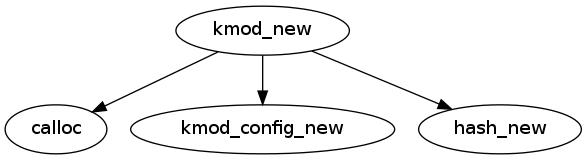
\includegraphics{./figures/kmod_new.jpg}
\caption{kmod\_new 调用层次图}
\end{figure}

\subsubsection{kmod\_unref() 核心代码分析}

{\begin{shaded}\begin{verbatim}
kmod_ctx *kmod_unref(kmod_ctx *ctx)
{
    kmod_unload_resources(ctx);
    hash_free(ctx->modules_by_name);
    kmod_config_free(ctx->config);
    free(ctx);

    return NULL;
}
\end{verbatim}\end{shaded}}
\begin{figure}[htbp]
\centering
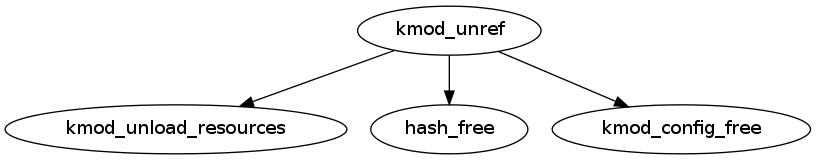
\includegraphics{./figures/kmod_unref.jpg}
\caption{kmod\_unref 调用层次图}
\end{figure}

\subsubsection{kmod\_module\_new\_from\_path() 核心代码分析}

{\begin{shaded}\begin{verbatim}
int kmod_module_new_from_path(kmod_ctx *ctx, char *path, kmod_module **mod)
{
    path_to_modname(path, name, &namelen);
    m = kmod_pool_get_module(ctx, name);
    kmod_module_ref(m);
    err = kmod_module_new(ctx, name, name, namelen, NULL, 0, &m); *
    *mod = m;
    return 0;
}
\end{verbatim}\end{shaded}}
\begin{figure}[htbp]
\centering
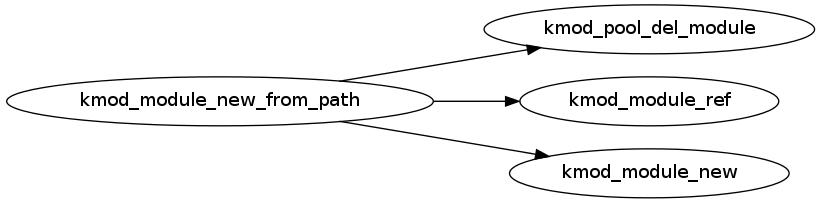
\includegraphics{./figures/kmod_module_new_from_path.jpg}
\caption{kmod\_module\_new\_from\_path 调用层次图}
\end{figure}

\subsubsection{kmod\_module\_insert\_module() 核心代码分析}

{\begin{shaded}\begin{verbatim}
int kmod_module_insert_module(kmod_module *mod, int flags, char *options)
{
    path = kmod_module_get_path(mod);
    file = kmod_file_open();
    size = kmod_file_get_size(file);
    mem = kmod_file_get_contents(file);
    elf = kmod_elf_new(mem, size);
    kmod_elf_strip_section(elf);
    mem = kmod_elf_get_memory(elf);
    init_module(mem, size, args);
    kmod_elf_unref(elf);
    kmod_file_unref(file);
}
\end{verbatim}\end{shaded}}
\begin{figure}[htbp]
\centering
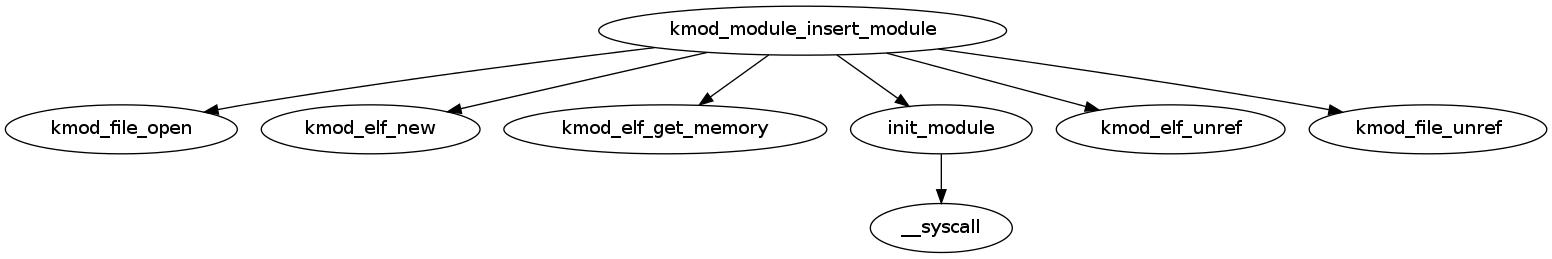
\includegraphics{./figures/kmod_module_insert_module.jpg}
\caption{kmod\_module\_insert\_module 调用层次图}
\end{figure}

\subsubsection{kmod\_module\_unref() 核心代码分析}

{\begin{shaded}\begin{verbatim}
kmod_module *kmod_module_unref(kmod_module *mod)
{
    --mod->refcount;

    kmod_pool_del_module(mod->ctx, mod, mod->hashkey);
    kmod_module_unref_list(mod->dep);
    kmod_file_unref(mod->file);
    kmod_unref(mod->ctx);

    return NULL;
}
\end{verbatim}\end{shaded}}
\begin{figure}[htbp]
\centering
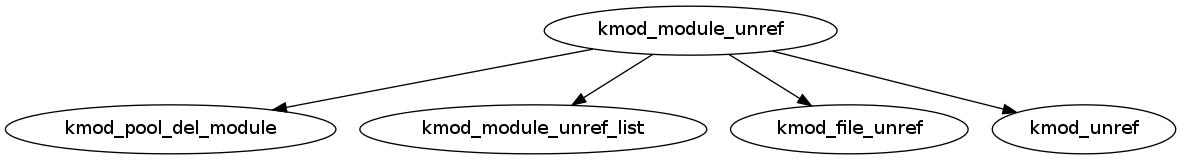
\includegraphics{./figures/kmod_module_unref.jpg}
\caption{kmod\_module\_unref 调用层次图}
\end{figure}

\subsubsection{init\_module() 核心代码分析}

{\begin{shaded}\begin{verbatim}
long init_module(void *mem, unsigned long len, const char *args)
{
    kmod_elf *elf = kmod_elf_new(mem, len);

    err = kmod_elf_get_section(elf, ".gnu.linkonce.this_module", &buf, &bufsize);
    kmod_elf_unref(elf);
    mod = find_module(modules, modname);
    if(mod != NULL)
    { 
    } else if (module_is_inkernel(modname))
    {
    } else
        create_sysfs_files(modname);

    return err;
}
\end{verbatim}\end{shaded}}
\subsubsection{do\_rmmod() 核心代码分析}

{\begin{shaded}\begin{verbatim}
do_rmmod(int argc, char *argv[])
{
    flags = argv[x];    // -f, -w, 
    ctx = kmod_new(NULL, &null_config);
    err = kmod_module_new_from_path(ctx, filename, &mod);
    err = kmod_module_remove_module(mod, flags);
    kmod_module_unref(mod);
    kmod_unref(ctx);
}
\end{verbatim}\end{shaded}}
\subsubsection{kmod\_module\_remove\_module() 核心代码分析}

{\begin{shaded}\begin{verbatim}
int kmod_module_remove_module(kmod_module *mod, int flags)
{
    err = delete_module(mod->name, flags);

    return err;
}
\end{verbatim}\end{shaded}}
\subsubsection{delete\_module() 核心代码分析}

{\begin{shaded}\begin{verbatim}
long init_module(void *mem, int flags)
{
    struct mod *mod;

    mod = find_module(modules, modname);

    return mod->ret;
}
\end{verbatim}\end{shaded}}

\end{document}
